\documentclass{ximera}

%\documentclass{ximera}

\usepackage{float}
\usepackage{subcaption}

\pgfplotsset{compat=1.16}

\newtheorem{ass}{Assumption}

\def\check{\tikz\fill[scale=0.4](0,.35) -- (.25,0) -- (1,.7) -- (.25,.15) -- cycle;}





\outcome{Learn about options that can be used as building blocks.}

\author{Brad Waller}

%Section 1.5

\title{Or-Nothing Options}

\begin{document}

\begin{abstract}
The cash-or-nothing and asset-or-nothing options can be used as building blocks for almost all of our derivatives. With a little creativity, they can be used to approximate almost any derivative!
\end{abstract}

\maketitle

In our section introducing calls and put, we saw that they had payoffs that are piecewise functions. We graphed the payoff diagram of a collection of these options and saw what a mess it could become, and it wasn't the easiest thing to produce. The benefit of ``Or-Nothing'' options is that they make graphs much easier to produce. In addition, they readily approximate payoffs of the most exotic of derivatives. 

\begin{definition}
An {\bf asset-or-nothing option} pays the underlying asset at expiration depending on whether it is a call or a put. A {\bf cash-or-nothing option} pays $\$1$ at expiration depending on whether it is a call or a put. 
\end{definition}

The payoffs for each of these four derivatives should be written explicitly. We will assume that these options are European throughout this text.

\begin{align*}
c_{\text{A/N}}\text{ has payoff }&
	\begin{cases}
	S(T)	&\text{ if } S(T)>K\\
	0	&\text{ otherwise,}
	\end{cases}\\
p_{\text{A/N}}\text{ has payoff } &
	\begin{cases}
	0	&\text{ if } S(T)>K\\
	S(T)	&\text{ otherwise,}
	\end{cases}\\
c_{\text{C/N}}\text{ has payoff } &
	\begin{cases}
	1	&\text{ if } S(T)>K\\
	0	&\text{ otherwise,}
	\end{cases}\\
p_{\text{C/N}}\text{ has payoff } &
	\begin{cases}
	0	&\text{ if } S(T)>K\\
	1	&\text{ otherwise.}
	\end{cases}
\end{align*}

Graphically, this would be 

\begin{center}
	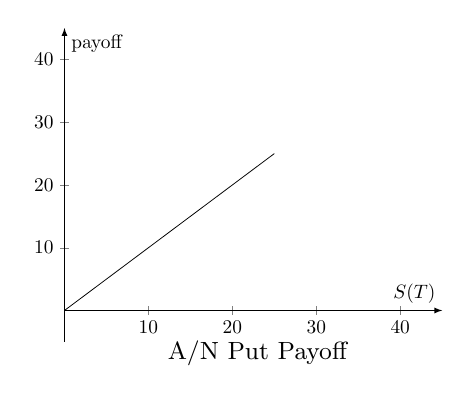
\begin{tikzpicture}[scale=0.7]
	\begin{axis}[
		xmin=0,
		xmax=45,
		%xtick={5,10,...,50},
		ymin=-5,
		ymax=45,
		%ytick={-20,-10,...,50},
		%grid=both,
		axis lines=middle,
		axis line style={->, >=latex},
		%x label style={at={(0.9,0.05)}},
		%x label style={at={(axis description cs:0.86,0.42)},anchor=north},
		xlabel={$S(T)$},
		ylabel={payoff}]
		%style={font=\tiny}]
		\addplot[black, smooth, domain=0:25, -, >=latex]{x};
	\end{axis}
	\node at (3.5, -0.2){\small A/N Put Payoff};
	\end{tikzpicture}
	\hspace{10pt}
	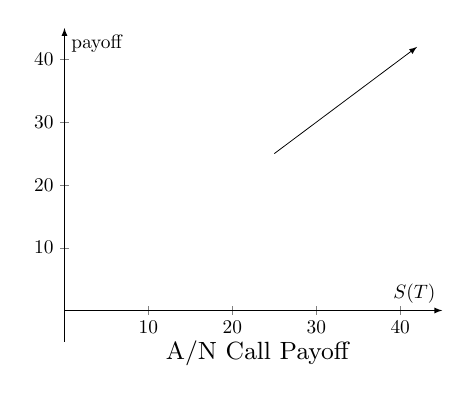
\begin{tikzpicture}[scale=0.7]
	\begin{axis}[
		xmin=0,
		xmax=45,
		%xtick={5,10,...,50},
		ymin=-5,
		ymax=45,
		%ytick={-20,-10,...,50},
		%grid=both,
		axis lines=middle,
		axis line style={->, >=latex},
		%x label style={at={(axis description cs:0.86,0.42)},anchor=north},
		xlabel={$S(T)$},
		ylabel={payoff}]
		%style={font=\tiny}]
		\addplot[black, smooth, domain=25:42, ->, >=latex]{x};
	\end{axis}
	\node at (3.5, -0.2){\small A/N Call Payoff};
	\end{tikzpicture}
\end{center}

and 

\begin{center}
	\begin{tikzpicture}[scale=0.7]
	\begin{axis}[
		xmin=0,
		xmax=45,
		%xtick={5,10,...,50},
		ymin=-2,
		ymax=3,
		%ytick={-20,-10,...,50},
		%grid=both,
		axis lines=middle,
		axis line style={->, >=latex},
		%x label style={at={(0.9,0.05)}},
		%x label style={at={(axis description cs:0.86,0.42)},anchor=north},
		xlabel={$S(T)$},
		ylabel={payoff}]
		%style={font=\tiny}
		\addplot[black, smooth, domain=0:25, -, >=latex]{1};
	\end{axis}
	\node at (3.5, -0.2){\small C/N Put Payoff};
	\end{tikzpicture}
	\hspace{10pt}
	\begin{tikzpicture}[scale=0.7]
	\begin{axis}[
		xmin=0,
		xmax=45,
		%xtick={5,10,...,50},
		ymin=-2,
		ymax=3,
		%ytick={-20,-10,...,50},
		%grid=both,
		axis lines=middle,
		axis line style={->, >=latex},
		%x label style={at={(axis description cs:0.86,0.42)},anchor=north},
		xlabel={$S(T)$},
		ylabel={payoff}]
		%style={font=\tiny}
		\addplot[black, smooth, domain=25:42, ->, >=latex]{1};
	\end{axis}
	\node at (3.5, -0.2){\small C/N Call Payoff};
	\end{tikzpicture}
\end{center}

The payoffs for these derivatives are quite simple, and it is for that reason that we use these options to approximations to complicated payoffs. There are three rules of thumb when dealing with these options:
\begin{enumerate}
\item To approximate nonzero slopes, use asset-or-nothing options.
\item To approximate zero slopes, use cash-or-nothing options.
\item To shift a diagram up or down, use cash-or-nothing options.
\end{enumerate}

Let's try an example!

\begin{example}
Suppose you have a derivative that has time $T$ payoff given by the function
	\begin{equation*}
	f(S)=
		\begin{cases}
		5& \text{if }S(T)\leq20,\\
		3S-55& \text{if } 20<S(T)\leq 25\\
		20 & \text{if }25<S(T).
		\end{cases}
	\end{equation*}
Construct a portfolio that will give you the exact payoff described by the function.
\end{example}

\begin{solution}
It should be clear where to use the various types of options based on our rules of thumb. The first and third pieces follow directly from the rules. For the first piece, it is probably best to use 5 cash-or-nothing puts with strike 20. For the third piece, it is probably best to use 20 cash-or-nothing calls with strike 25. 

The middle piece requires the most thought. The rule of thumb tells us that when slope is involved, we should use asset-or-nothing options. Here, the slope is 3. It follows that we should buy 3 asset-or-nothing calls with strike 20. What is not clear, is that we need to cancel out the payoff of these three calls after the value 25 (otherwise we would interfere with the third piece). To make the appropriate cancellation, we write three asset-or-nothing calls with strike 25. We are close to the desired payoff. The slope is right, but the location is not. We must shift the diagram down!

We use the last rule of thumb. If we use the value $S(T)=20$ with our asset-or-nothing options as an anchor point, we see that the payoff value is $60$. We need to shift our diagram down by 55!. To do this, write 55 cash-or-nothing calls with strike 20 and purchase 55 cash-or-nothing calls with strike 25.

The required portfolio is as follows:
\begin{itemize}
\item 5 cash-or-nothing puts with $K=20$,
\item 20 cash-or-nothing calls with $K=25$,
\item 3 asset-or-nothing calls with $K=20$,
\item 3 written asset-or-nothing calls with $K=25$,
\item 55 written cash-or-nothing calls with $K=20$,
\item and 55 cash-or-nothing calls with $K=25$.
\end{itemize}
We could go further by combining like terms, but I'll leave that to you in your spare time!

\end{solution}

Why don't you try to work through a similar problem.

\begin{question}
Select all of the following that will produce the payoff described by the function
	\begin{equation*}
	f(S)=
		\begin{cases}
		2(S-20) & \text{if } 20<S(T)\leq 30\\
		0 & \text{otherwise.}
		\end{cases}
	\end{equation*}
For a greater challenge, try this problem before seeing the options below. Your answer may be correct, but it might look different than the options given.
	\begin{selectAll}
		\choice{Two asset-or-nothing calls with strike 20}
		\choice[correct]{Two asset-or-nothing puts with strike 30}
		\choice[correct]{Forty cash-or-nothing calls with strike 30}
		\choice{Two written asset-or-nothing calls with strike 25}
		\choice[correct]{Two written asset-or-nothing puts with strike 20}
		\choice{Forty cash-or-nothing puts with strike 30}
		\choice[correct]{Forty written cash-or-nothing calls with strike 20}
	\end{selectAll}
\end{question}

\begin{solution}
It is clear that there should be two asset-or-nothing options from our rules. The only pair that have the appropriate values are the asset-or-nothing puts. If you try to graph the position of these two types of options, you will see that the function is forty units too high! We must shift down by 40 using the cash-or-nothing options. Writing 40 cash-or-nothing calls with strike 20 and purchasing 40 cash-or-nothing calls with strike 30 accomplishes this.
\end{solution}

\begin{remark}
In our definitions of the or-nothing options, it was specified that $S(T)>K$ in the conditions. This makes these functions left-continuous. I won't expect you to remember this specific of a detail. Because of this, you won't need to worry if the endpoints in your graphs need hollow dots or filled in dots (unless you choose to). The reason I don't require you to remember this detail is that when we deal with continuous probabilities in the future, the value of these functions at one point will not change the price of the derivatives in question.
\end{remark}




\end{document}



